\documentclass[border=10pt,tikz]{standalone}
\usepackage{tikz}
\usetikzlibrary{positioning,arrows.meta,shapes}
\begin{document}
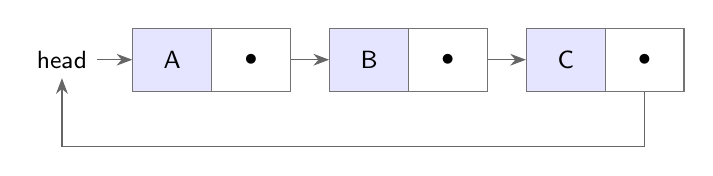
\begin{tikzpicture}[
  font=\sffamily\small,
  node/.style={rectangle, draw=black!55, line width=0.4pt, minimum height=8mm,
               inner sep=0pt, fill=blue!10},
  cell/.style={node, minimum width=10mm, align=center},
  arr/.style={-{Stealth[length=2mm]}, draw=black!60}
]
% head label
\node (h) at (-3, 0) {head};

% A node
\node[cell] (a1) at (-1.6, 0) {A};
\node[cell, fill=white] (a2) at (-0.6, 0) {$\bullet$};

% B node
\node[cell] (b1) at (0.9, 0) {B};
\node[cell, fill=white] (b2) at (1.9, 0) {$\bullet$};

% C node
\node[cell] (c1) at (3.4, 0) {C};
\node[cell, fill=white] (c2) at (4.4, 0) {$\bullet$};

\draw[arr] (h.east) -- (a1.west);
\draw[arr] (a2.east) -- (b1.west);
\draw[arr] (b2.east) -- (c1.west);

% circular back link
\draw[arr] (c2.south) -- ++(0,-0.7) -| (h.south);
\end{tikzpicture}
\end{document}
